\documentclass[aspectratio=169,11pt]{beamer}
\usetheme{metropolis}
\usepackage{tikz}
\usetikzlibrary{arrows.meta,positioning,calc}
\usepackage{booktabs}
\usepackage{xcolor}
\usepackage{amsmath}
\usepackage{textcomp}
\usepackage{array}
\usepackage{hyperref}

% === Color palette ===
\definecolor{report}{HTML}{3498DB}
\definecolor{state}{HTML}{9B59B6}
\definecolor{bias}{HTML}{E67E22}
\definecolor{neutral}{HTML}{95A5A6}
\definecolor{pass}{HTML}{27AE60}
\definecolor{fail}{HTML}{E74C3C}
\tikzset{
  box/.style={draw=#1,thick,rounded corners,fill=#1!10,minimum width=3.2cm,minimum height=0.9cm,font=\small,align=center},
  boxL/.style={draw=#1,thick,rounded corners,fill=#1!10,minimum width=5.2cm,minimum height=1.2cm,font=\small,align=center},
  boxS/.style={draw=#1,thick,rounded corners,fill=#1!10,minimum width=2.8cm,minimum height=0.9cm,font=\footnotesize,align=center},
  panel/.style={draw=#1,thick,rounded corners,fill=#1!8},
}
\hypersetup{colorlinks=true,linkcolor=.,urlcolor=report}
\hyphenpenalty=10000
\exhyphenpenalty=10000

\title{Measurement Without a Trusted Instrument}
\subtitle{Hasok Chang's epistemic iteration and Eran Tal's model-based measurement, applied to AI introspection}
\author{Measuring AI Self-Reports}
\date{}
\institute{}

\newcommand{\partslide}[2]{%
\begin{frame}[plain,label=#1]
\vfill
\begin{center}
  \setlength{\fboxrule}{2.5pt}%
  \fcolorbox{black}{white}{\parbox{0.65\textwidth}{\centering\vspace{0.8em}
    {\Large\bfseries #2}
  \vspace{0.8em}}}
\end{center}
\vfill
\end{frame}}

\begin{document}

\begin{frame}[plain]\vspace*{-1.5em}\titlepage\end{frame}

%% --- Overview ---
\begin{frame}{Overview}\footnotesize\vspace*{-0.8em}
\begin{columns}[T]
\begin{column}{0.48\textwidth}
\hyperlink{part1}{\textbf{Part 1: The problem}}\\[0.1em]
{\scriptsize%
\quad\hyperlink{nothermo}{1.~A thermometer with nothing to check it against}\\%
\quad\hyperlink{llm}{2.~The same situation in a language model}\\%
\quad\hyperlink{answers}{3.~Three answers}%
}\vspace{0.25em}

\hyperlink{part2}{\textbf{Part 2: Chang, building temperature}}\\[0.1em]
{\scriptsize%
\quad\hyperlink{fixed}{4.~Fixed points}\\%
\quad\hyperlink{nomic}{5.~The problem of nomic measurement}\\%
\quad\hyperlink{compar}{6.~Comparability}\\%
\quad\hyperlink{single}{7.~The principle of single value}\\%
\quad\hyperlink{iter}{8.~Epistemic iteration}\\%
\quad\hyperlink{progress}{9.~Two kinds of progress}\\%
\quad\hyperlink{inaccurate}{10.~Calibration against an inaccurate standard}\\%
\quad\hyperlink{extension}{11.~Metrological extension}%
}
\end{column}
\begin{column}{0.48\textwidth}
\hyperlink{part3}{\textbf{Part 3: Tal, measurement as inference}}\\[0.1em]
{\scriptsize%
\quad\hyperlink{indication}{12.~Indication and outcome}\\%
\quad\hyperlink{calib}{13.~Three kinds of calibration}\\%
\quad\hyperlink{grc}{14.~The generalized robustness condition}\\%
\quad\hyperlink{individ}{15.~Quantity individuation}\\%
\quad\hyperlink{cesium}{16.~The cesium clock}%
}\vspace{0.25em}

\hyperlink{part4}{\textbf{Part 4: AI introspection}}\\[0.1em]
{\scriptsize%
\quad\hyperlink{taltable}{17.~Tal's terms in an introspection experiment}\\%
\quad\hyperlink{consequences}{18.~Scoring and scope}\\%
\quad\hyperlink{changmodel}{19.~Fixed points and comparability in a model}\\%
\quad\hyperlink{itermodel}{20.~Iteration in a model}\\%
\quad\hyperlink{extmodel}{21.~Extending ``introspection'' to models}\\%
\quad\hyperlink{limits}{22.~Where the analogy stops}\\%
\quad\hyperlink{summary}{23.~Summary}\\%
\quad\hyperlink{reading}{24.~Reading}%
}
\end{column}
\end{columns}
\end{frame}

%% ============================================================
\partslide{part1}{Part 1\\[0.5em]{\large\mdseries The problem: no trusted thermometer}}
%% ============================================================

\begin{frame}[label=nothermo]{A thermometer with nothing to check it against}
How do we know a thermometer reads the temperature correctly? The obvious test is to compare it with a thermometer we already trust. Early thermometry had no such thermometer.

\vspace{0.5em}
\begin{center}
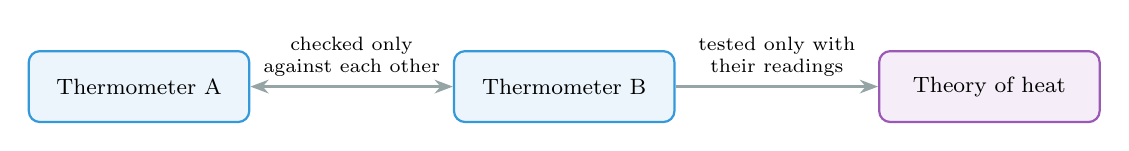
\begin{tikzpicture}
  \node[boxS=report] (a) at (0,0) {Thermometer A};
  \node[boxS=report] (b) at (5.4,0) {Thermometer B};
  \node[boxS=state] (t) at (10.8,0) {Theory of heat};
  \draw[{Stealth}-{Stealth},thick,neutral] (a) -- node[above,font=\scriptsize,text=black,align=center]{checked only\\against each other} (b);
  \draw[-{Stealth},thick,neutral] (b) -- node[above,font=\scriptsize,text=black,align=center]{tested only with\\their readings} (t);
\end{tikzpicture}
\end{center}

\vspace{0.5em}
{\small Every way of checking the instrument seems to need an instrument that does not yet exist.
\href{https://academic.oup.com/book/5530}{Hasok Chang's \emph{Inventing Temperature}} (2004) is the history of how thermometry was built anyway.
\href{https://plato.stanford.edu/entries/measurement-science/}{Eran Tal's model-based account} explains what calibration does when there is no independent access to the quantity.}
\end{frame}

\begin{frame}[label=llm]{The same situation in a language model}
The AI version is the \textbf{concept-injection} experiment:

\vspace{0.1em}
\begin{enumerate}\setlength\itemsep{1pt}
  \item {\small Take a vector for a word such as \emph{bread}.}
  \item {\small Add it to the model's activations while it answers.}
  \item {\small Ask the model whether it detects an injected thought, and what it is about.}
\end{enumerate}

\vspace{0.3em}
\begin{center}
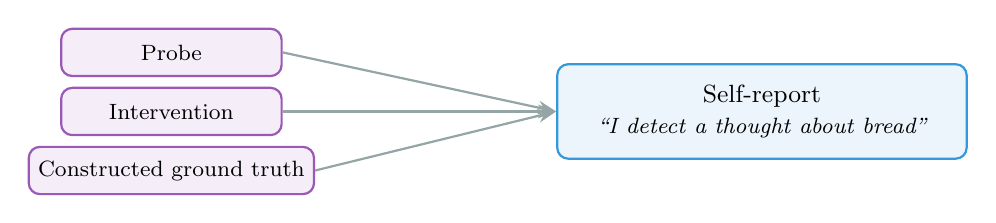
\begin{tikzpicture}
  \node[boxS=state,minimum height=0.6cm] (p) at (0,0.75) {Probe};
  \node[boxS=state,minimum height=0.6cm] (i) at (0,0) {Intervention};
  \node[boxS=state,minimum height=0.6cm] (g) at (0,-0.75) {Constructed ground truth};
  \node[boxL=report] (r) at (7.5,0) {Self-report\\{\footnotesize\itshape ``I detect a thought about bread''}};
  \draw[-{Stealth},thick,neutral] (p.east) -- (r.west);
  \draw[-{Stealth},thick,neutral] (i.east) -- (r.west);
  \draw[-{Stealth},thick,neutral] (g.east) -- (r.west);
\end{tikzpicture}
\end{center}

{\small No instrument for reading a model's internal states is already trusted. Each instrument the report can be checked against is itself still being developed.}
\end{frame}

\begin{frame}[label=answers]{Three answers}
Three bodies of work answer the question of how to trust an instrument without an independent ground truth.

\begin{center}
{\footnotesize\renewcommand{\arraystretch}{1.05}
\begin{tabular}{p{3.2cm}>{\raggedright\arraybackslash}p{9.6cm}}
\toprule
\textbf{Account} & \textbf{What does the justifying} \\
\midrule
\textcolor{report}{\textbf{Model-based (Tal)}} & The model of the measurement process. An outcome is inferred from an indication through that model, and trust comes from coherence across a network of instruments. \\
\textcolor{state}{\textbf{Iteration (Chang)}} & The history of corrections. Start from a standard accepted without proof and correct it through the inquiries it makes possible. \\
\textcolor{bias}{\textbf{Robustness}} & The independence of the procedures. Agreement among independent procedures is evidence that a result is real. \\
\bottomrule
\end{tabular}
}
\end{center}

\vspace{0.2em}
{\small All three agree that no measurement is justified from a foundation outside all theory. This deck covers the first two.}
\end{frame}

%% ============================================================
\partslide{part2}{Part 2\\[0.5em]{\large\mdseries Chang: building temperature}}
%% ============================================================

\begin{frame}[label=fixed]{Fixed points}
To mark a scale on a thermometer you need \textbf{fixed points}: phenomena that always happen at the same temperature.

\vspace{0.5em}
{\small Early thermometry had none that were agreed on, and no way to check a proposed fixed point without a thermometer already trusted.}

\vspace{0.4em}
\begin{center}
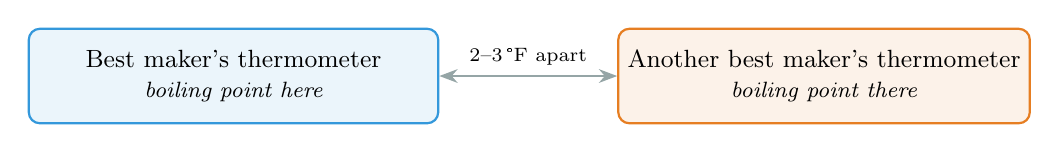
\begin{tikzpicture}
  \node[boxL=report] (a) at (0,0) {Best maker's thermometer\\{\footnotesize\itshape boiling point here}};
  \node[boxL=bias] (b) at (7.5,0) {Another best maker's thermometer\\{\footnotesize\itshape boiling point there}};
  \draw[{Stealth}-{Stealth},thick,neutral] (a) -- node[above,font=\scriptsize,text=black]{2--3\,\textdegree F apart} (b);
\end{tikzpicture}
\end{center}

\vspace{0.6em}
Even boiling water was not fixed. In 1776 a Royal Society committee found that thermometers from the best makers disagreed on the boiling point by 2--3\,\textdegree F.
\end{frame}

\begin{frame}[label=nomic]{The problem of nomic measurement}
Thermometers of mercury, alcohol and water, calibrated at the same fixed points, disagree. Which fluid expands uniformly?

\begin{center}
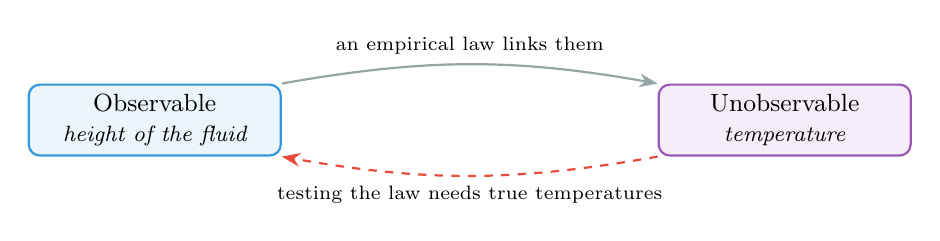
\begin{tikzpicture}
  \node[box=report] (y) at (0,0) {Observable\\{\footnotesize\itshape height of the fluid}};
  \node[box=state] (x) at (8,0) {Unobservable\\{\footnotesize\itshape temperature}};
  \draw[-{Stealth},thick,neutral] (y.north east) to[bend left=10] node[above,font=\scriptsize,text=black]{an empirical law links them} (x.north west);
  \draw[-{Stealth},thick,dashed,fail] (x.south west) to[bend left=10] node[below,font=\scriptsize,text=black]{testing the law needs true temperatures} (y.south east);
\end{tikzpicture}
\end{center}
\vspace{-0.4em}

{\small Chang generalizes: when a measurement rests on a law linking an observable to an unobservable quantity, testing the law needs the very measurement it is supposed to justify.}

{\small Tal's \href{https://plato.stanford.edu/entries/measurement-science/}{encyclopedia entry} places it beside van Fraassen's \textbf{problem of coordination}: which procedure measures a quantity and what the quantity is cannot be settled separately.}
\end{frame}

\begin{frame}[label=compar]{Comparability}
In the 1840s Regnault tested thermometers without assuming any theory of heat. His criterion was \textbf{comparability}: a thermometer that reads the true temperature must at least give the same reading in the same circumstance, and all thermometers of one type must agree with each other.

\vspace{0.6em}
\begin{columns}[T]
\begin{column}{0.48\textwidth}
\begin{center}
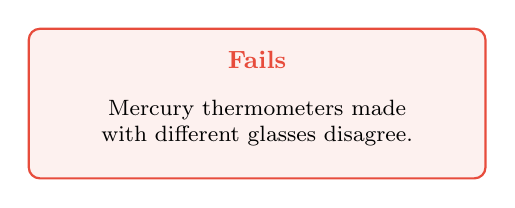
\begin{tikzpicture}
  \draw[panel=fail] (0,0) rectangle (5.8,1.9);
  \node[font=\small\bfseries,fail] at (2.9,1.5) {Fails};
  \node[font=\footnotesize,align=center,text width=5.3cm] at (2.9,0.7) {Mercury thermometers made with different glasses disagree.};
\end{tikzpicture}
\end{center}
\end{column}
\begin{column}{0.48\textwidth}
\begin{center}
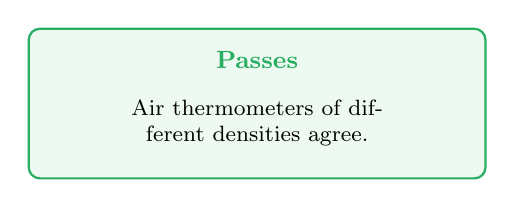
\begin{tikzpicture}
  \draw[panel=pass] (0,0) rectangle (5.8,1.9);
  \node[font=\small\bfseries,pass] at (2.9,1.5) {Passes};
  \node[font=\footnotesize,align=center,text width=5.3cm] at (2.9,0.7) {Air thermometers of different densities agree.};
\end{tikzpicture}
\end{center}
\end{column}
\end{columns}

\vspace{0.6em}
{\small Regnault never treated comparability as truth: air thermometers passing did not show that they read the true temperature.}
\end{frame}

\begin{frame}[label=single]{The principle of single value}
Chang names the assumption behind comparability: \emph{``a real physical property can have no more than one definite value in a given situation.''}

\vspace{0.1em}
{\small The principle is neither logical nor empirical, and no observation could test it. Regnault's test was \textbf{minimalist}: he compared thermometers of one type against each other and added no hypotheses about heat, so a failure could be blamed only on the thermometers.}

\vspace{0.1em}
\begin{center}
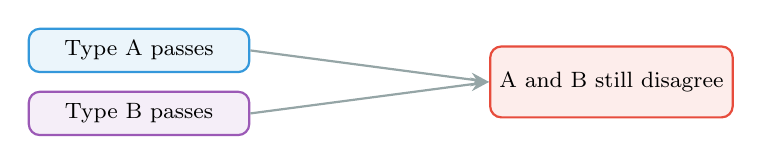
\begin{tikzpicture}
  \node[boxS=report,minimum height=0.55cm] (a) at (0,0.4) {Type A passes};
  \node[boxS=state,minimum height=0.55cm] (b) at (0,-0.4) {Type B passes};
  \node[boxS=fail] (d) at (6,0) {A and B still disagree};
  \draw[-{Stealth},thick,neutral] (a.east) -- (d.west);
  \draw[-{Stealth},thick,neutral] (b.east) -- (d.west);
\end{tikzpicture}
\end{center}

{\small The limit: several types can each pass the comparability test and still disagree with each other. Minimalism strengthens a verdict when there is one, but cannot guarantee a verdict.}
\end{frame}

\begin{frame}[label=iter]{Epistemic iteration}
Chang's answer to the circle: start from an existing system of knowledge, accepted without proof that it is correct, and use it to run inquiries that refine and correct it.

\vspace{0.5em}
\begin{center}
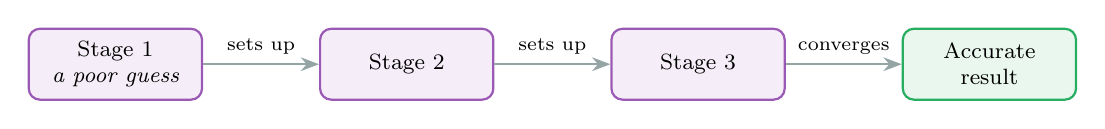
\begin{tikzpicture}
  \node[boxS=state,minimum width=2.2cm] (s1) at (0,0) {Stage 1\\{\footnotesize\itshape a poor guess}};
  \node[boxS=state,minimum width=2.2cm] (s2) at (3.7,0) {Stage 2};
  \node[boxS=state,minimum width=2.2cm] (s3) at (7.4,0) {Stage 3};
  \node[boxS=pass,minimum width=2.2cm] (s4) at (11.1,0) {Accurate\\result};
  \draw[-{Stealth},thick,neutral] (s1) -- node[above,font=\scriptsize,text=black]{sets up} (s2);
  \draw[-{Stealth},thick,neutral] (s2) -- node[above,font=\scriptsize,text=black]{sets up} (s3);
  \draw[-{Stealth},thick,neutral] (s3) -- node[above,font=\scriptsize,text=black]{converges} (s4);
\end{tikzpicture}
\end{center}

\vspace{0.5em}
{\small Chang's example is a reconstruction of how Fahrenheit could have set the temperature of his mixing vessel: start from a poor guess and let each trial set up the next, converging on an accurate result.}

\vspace{0.3em}
{\small The circularity cannot be escaped, so justification in empirical science has to be coherentist. What justifies the result is the self-correcting progress, not a secure foundation.}
\end{frame}

\begin{frame}[label=progress]{Two kinds of progress}
\begin{columns}[T]
\begin{column}{0.48\textwidth}
\begin{center}
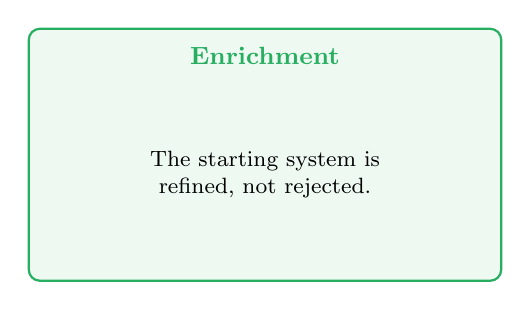
\begin{tikzpicture}
  \draw[panel=pass] (0,0) rectangle (6,3.2);
  \node[font=\small\bfseries,pass] at (3,2.85) {Enrichment};
  \node[font=\footnotesize,align=center,text width=5.5cm] at (3,1.35) {The starting system is refined, not rejected.};
\end{tikzpicture}
\end{center}
\end{column}
\begin{column}{0.48\textwidth}
\begin{center}
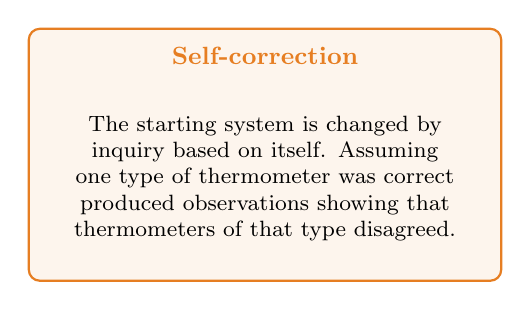
\begin{tikzpicture}
  \draw[panel=bias] (0,0) rectangle (6,3.2);
  \node[font=\small\bfseries,bias] at (3,2.85) {Self-correction};
  \node[font=\footnotesize,align=center,text width=5.5cm] at (3,1.3) {The starting system is changed by inquiry based on itself. Assuming one type of thermometer was correct produced observations showing that thermometers of that type disagreed.};
\end{tikzpicture}
\end{center}
\end{column}
\end{columns}

\vspace{0.7em}
\begin{itemize}\setlength\itemsep{4pt}
  \item {\small Nothing guarantees that iteration succeeds. If every attempt to improve a system contradicts itself, the system has failed.}
  \item {\small Competing traditions can progress in parallel, each on its own basis.}
\end{itemize}
\end{frame}

\begin{frame}[label=inaccurate]{Calibration against an inaccurate standard}
An objection: a procedure cannot be calibrated without an accurate one. \href{https://philpapers.org/archive/MICCIC-2.pdf}{Matthias Michel (2021)} answers it with Chang's history.

\vspace{0.5em}
\begin{center}
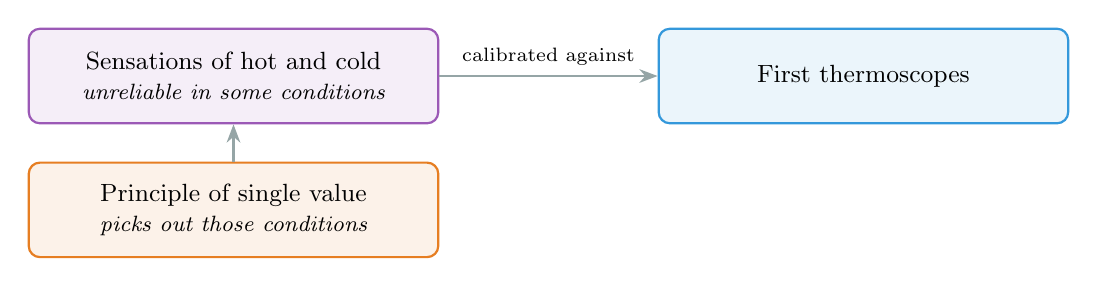
\begin{tikzpicture}
  \node[boxL=state] (s) at (0,0) {Sensations of hot and cold\\{\footnotesize\itshape unreliable in some conditions}};
  \node[boxL=report] (t) at (8,0) {First thermoscopes};
  \node[boxL=bias] (p) at (0,-1.7) {Principle of single value\\{\footnotesize\itshape picks out those conditions}};
  \draw[-{Stealth},thick,neutral] (s) -- node[above,font=\scriptsize,text=black]{calibrated against} (t);
  \draw[-{Stealth},thick,neutral] (p) -- (s);
\end{tikzpicture}
\end{center}

\vspace{0.2em}
{\small The first thermoscopes were calibrated against human sensations of hot and cold, which were known to be unreliable in some conditions. The principle of single value picked out those conditions. Inaccurate procedures are not useless.}
\end{frame}

\begin{frame}[label=extension]{Metrological extension}
Temperature measurement was carried into extreme cold and heat, where mercury froze and glass melted. Chang calls carrying a measurement method into a new domain \textbf{metrological extension}.

{\small The method is valid if it coheres with the rest of the concept's meaning. Two conditions:}

\begin{columns}[T]
\begin{column}{0.48\textwidth}
\begin{center}
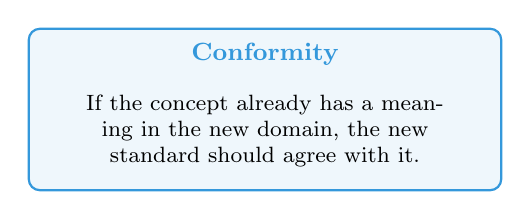
\begin{tikzpicture}
  \draw[panel=report] (0,0) rectangle (6,2.05);
  \node[font=\small\bfseries,report] at (3,1.72) {Conformity};
  \node[font=\footnotesize,align=center,text width=5.5cm] at (3,0.75) {If the concept already has a meaning in the new domain, the new standard should agree with it.};
\end{tikzpicture}
\end{center}
\end{column}
\begin{column}{0.48\textwidth}
\begin{center}
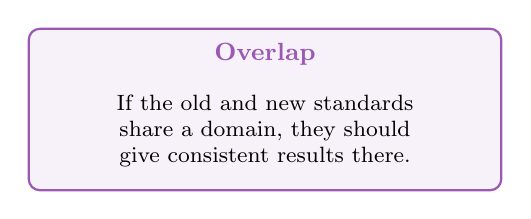
\begin{tikzpicture}
  \draw[panel=state] (0,0) rectangle (6,2.05);
  \node[font=\small\bfseries,state] at (3,1.72) {Overlap};
  \node[font=\footnotesize,align=center,text width=5.5cm] at (3,0.75) {If the old and new standards share a domain, they should give consistent results there.};
\end{tikzpicture}
\end{center}
\end{column}
\end{columns}

\vspace{0.1em}
{\footnotesize \href{https://580d4178-4a2a-40ee-b753-91905f0859e6.filesusr.com/ugd/b898ea_5e898d22d16b4ba89c07c379485770ed.pdf}{Michel (2024)} adds an \textbf{existence condition} (the construct must be present in the new domain) and requires the shared domain. When the conditions fail, a validity drift can follow.}
\end{frame}

%% ============================================================
\partslide{part3}{Part 3\\[0.5em]{\large\mdseries Tal: measurement as inference}}
%% ============================================================

\begin{frame}[label=indication]{Indication and outcome}
\href{https://plato.stanford.edu/entries/measurement-science/}{Tal's} measurement has two levels: a concrete process in which object, instrument and environment interact, and an abstract model of that process.

\vspace{0.2em}
\begin{center}
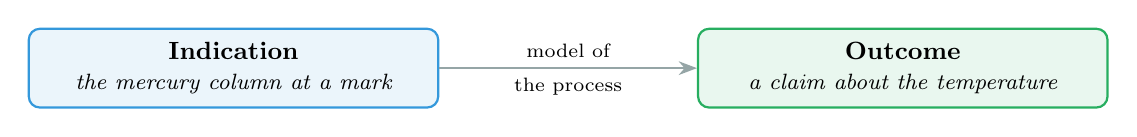
\begin{tikzpicture}
  \node[boxL=report,minimum height=1cm] (i) at (0,0) {\textbf{Indication}\\{\footnotesize\itshape the mercury column at a mark}};
  \node[boxL=pass,minimum height=1cm] (o) at (8.5,0) {\textbf{Outcome}\\{\footnotesize\itshape a claim about the temperature}};
  \draw[-{Stealth},thick,neutral] (i) -- node[above,font=\scriptsize,text=black]{model of} node[below,font=\scriptsize,text=black]{the process} (o);
\end{tikzpicture}
\end{center}

\begin{itemize}\setlength\itemsep{1pt}
  \item {\small An \textbf{\textcolor{report}{indication}} is a property of the instrument in its final state: a pointer position, a number, a symbol or any other output.}
  \item {\small An \textbf{\textcolor{pass}{outcome}} is a knowledge claim about the object, inferred from indications together with background knowledge.}
  \item {\small Without the model there is no outcome. The same indications can support different outcomes under different models.}
\end{itemize}
\end{frame}

\begin{frame}[label=calib]{Three kinds of calibration}
For \href{https://philpapers.org/rec/TALCMT}{Tal (2017)}, calibration is modeling: building models of the measurement process, deriving predictions and testing them.

\begin{center}
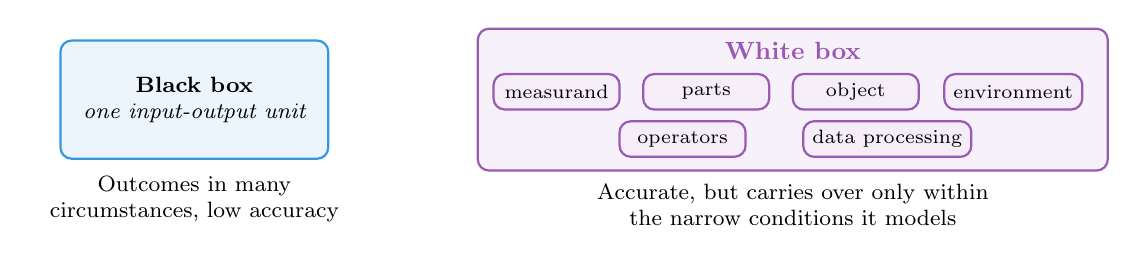
\begin{tikzpicture}
  \node[boxS=report,minimum width=3.4cm,minimum height=1.5cm] (bb) at (0,0) {\textbf{Black box}\\{\footnotesize\itshape one input-output unit}};
  \node[font=\footnotesize,align=center,text width=4cm,anchor=north] at (0,-0.85) {Outcomes in many\\circumstances, low accuracy};
  \draw[panel=state] (3.6,-0.9) rectangle (11.6,0.9);
  \node[font=\small\bfseries,state] at (7.6,0.62) {White box};
  \node[boxS=state,minimum width=1.6cm,minimum height=0.45cm,font=\scriptsize] at (4.6,0.1) {measurand};
  \node[boxS=state,minimum width=1.6cm,minimum height=0.45cm,font=\scriptsize] at (6.5,0.1) {parts};
  \node[boxS=state,minimum width=1.6cm,minimum height=0.45cm,font=\scriptsize] at (8.4,0.1) {object};
  \node[boxS=state,minimum width=1.6cm,minimum height=0.45cm,font=\scriptsize] at (10.4,0.1) {environment};
  \node[boxS=state,minimum width=1.6cm,minimum height=0.45cm,font=\scriptsize] at (6.2,-0.5) {operators};
  \node[boxS=state,minimum width=1.6cm,minimum height=0.45cm,font=\scriptsize] at (8.8,-0.5) {data processing};
  \node[font=\footnotesize,align=center,text width=7.5cm,anchor=north] at (7.6,-0.95) {Accurate, but carries over only within\\the narrow conditions it models};
\end{tikzpicture}
\end{center}

{\small \textbf{Coherent calibration} models the process so that it fits background knowledge and applies the quantity consistently across objects, procedures and conditions. Black-box and white-box calibration are special cases of it.}
\end{frame}

\begin{frame}[label=grc]{The generalized robustness condition}
Calibration cannot test outcomes independently of every background assumption. It can test them across a network of instruments.

\vspace{0.1em}
\begin{center}
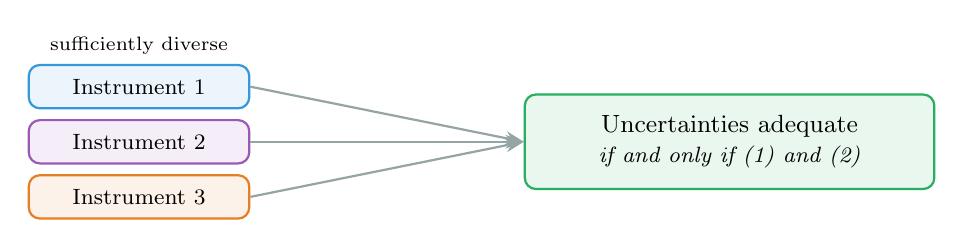
\begin{tikzpicture}
  \node[boxS=report,minimum height=0.55cm] (a) at (0,0.7) {Instrument 1};
  \node[boxS=state,minimum height=0.55cm] (b) at (0,0) {Instrument 2};
  \node[boxS=bias,minimum height=0.55cm] (c) at (0,-0.7) {Instrument 3};
  \node[font=\scriptsize,text=black,anchor=south] at (a.north) {sufficiently diverse};
  \node[boxL=pass] (o) at (7.5,0) {Uncertainties adequate\\{\footnotesize\itshape if and only if (1) and (2)}};
  \draw[-{Stealth},thick,neutral] (a.east) -- (o.west);
  \draw[-{Stealth},thick,neutral] (b.east) -- (o.west);
  \draw[-{Stealth},thick,neutral] (c.east) -- (o.west);
\end{tikzpicture}
\end{center}

\begin{enumerate}\setlength\itemsep{0pt}
  \item {\small Their outcomes agree within those uncertainties.}
  \item {\small Each uncertainty comes from an adequate model of its process.}
\end{enumerate}

{\small Calibration cannot verify outcomes independently of any model, but it can verify them independently of any \emph{particular} model, instrument and environment.}
\end{frame}

\begin{frame}[label=individ]{Quantity individuation}
When do two procedures measure the same quantity? \href{https://philpapers.org/rec/TALIQ}{Tal (2019)}: when their outcomes disagree, three explanations compete.

\vspace{0.2em}
\begin{center}
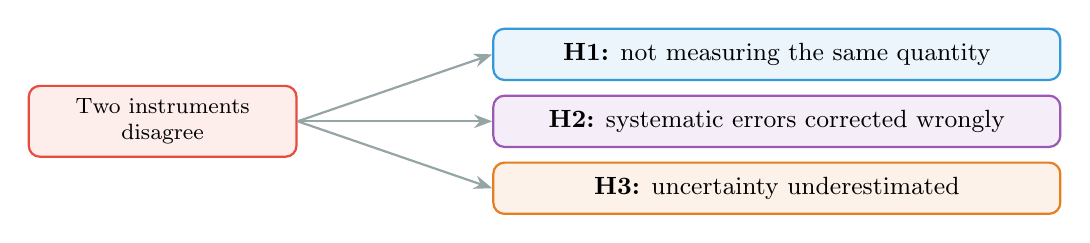
\begin{tikzpicture}
  \node[boxS=fail,minimum width=3.4cm] (d) at (0,0) {Two instruments\\disagree};
  \node[boxL=report,minimum width=7.2cm,minimum height=0.65cm] (h1) at (7.8,0.85) {\textbf{H1:} not measuring the same quantity};
  \node[boxL=state,minimum width=7.2cm,minimum height=0.65cm] (h2) at (7.8,0) {\textbf{H2:} systematic errors corrected wrongly};
  \node[boxL=bias,minimum width=7.2cm,minimum height=0.65cm] (h3) at (7.8,-0.85) {\textbf{H3:} uncertainty underestimated};
  \draw[-{Stealth},thick,neutral] (d.east) -- (h1.west);
  \draw[-{Stealth},thick,neutral] (d.east) -- (h2.west);
  \draw[-{Stealth},thick,neutral] (d.east) -- (h3.west);
\end{tikzpicture}
\end{center}

\vspace{0.1em}
{\small These cannot be tested one at a time. Establishing what instruments measure, how accurate they are and whether they agree are entangled tasks, and no context-free rule settles the choice.}

\vspace{0.1em}
{\small Tal's criterion: two procedures measure the same quantity if both can be modeled coherently in terms of the same type of quantity in the background theory.}
\end{frame}

\begin{frame}[label=cesium]{The cesium clock}
One route to that criterion is \textbf{unity through idealization}: different concrete circumstances measure the same quantity if they are modeled as approximations of the same ideal circumstance.

\vspace{0.5em}
\begin{center}
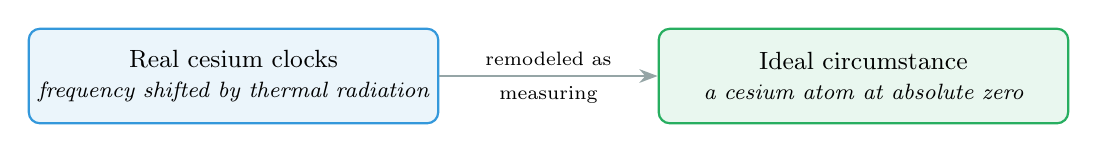
\begin{tikzpicture}
  \node[boxL=report] (c) at (0,0) {Real cesium clocks\\{\footnotesize\itshape frequency shifted by thermal radiation}};
  \node[boxL=pass] (i) at (8,0) {Ideal circumstance\\{\footnotesize\itshape a cesium atom at absolute zero}};
  \draw[-{Stealth},thick,neutral] (c) -- node[above,font=\scriptsize,text=black]{remodeled as} node[below,font=\scriptsize,text=black]{measuring} (i);
\end{tikzpicture}
\end{center}

\vspace{0.5em}
{\small When thermal radiation was found to shift the clocks' frequency, they were remodeled as measuring the frequency of a cesium atom at absolute zero.}

\vspace{0.3em}
{\small On this view, systematic error is what lets different instruments be modeled as measuring one quantity despite stable disagreements among their readings.}
\end{frame}

%% ============================================================
\partslide{part4}{Part 4\\[0.5em]{\large\mdseries AI introspection}}
%% ============================================================

\begin{frame}[label=taltable]{Tal's terms in an introspection experiment}
\begin{center}
{\footnotesize\renewcommand{\arraystretch}{1.1}
\begin{tabular}{p{3.4cm}>{\raggedright\arraybackslash}p{9.6cm}}
\toprule
\textbf{Model-based term} & \textbf{In a concept-injection experiment} \\
\midrule
Indication & The model's reply: yes or no, a named concept, a confidence number, a free-text description \\
Outcome & The claim that the model has access to, or represents, a given internal state \\
Model of the process & Assumptions about prompting, sampling, the judge, the intervention, and the route from internal state to reply \\
Black-box calibration & Fitting reply rates to a constructed ground truth, such as injected versus not injected, without modeling how the reply is produced \\
White-box calibration & Modeling the report pathway itself, for instance by mechanistic analysis of the circuit that produces the reply \\
H1 / H2 / H3 & When a self-report and a probe disagree: different quantities, uncorrected bias, or understated uncertainty \\
\bottomrule
\end{tabular}
}
\end{center}
\end{frame}

\begin{frame}[label=consequences]{Scoring and scope}
\begin{columns}[T]
\begin{column}{0.48\textwidth}
{\small\textbf{Scoring is part of the model}}\\[0.3em]
{\footnotesize The same indications support different outcomes under different models. A grader that credits any report of an anomaly and a grader that requires the correct concept turn the same replies into different outcomes.}
\end{column}
\begin{column}{0.48\textwidth}
{\small\textbf{A calibration holds where it was done}}\\[0.3em]
{\footnotesize A calibration against injected vectors at one layer and strength carries over, on Tal's account, only within the conditions under which it was made.}
\end{column}
\end{columns}

\vspace{0.2em}
\begin{center}
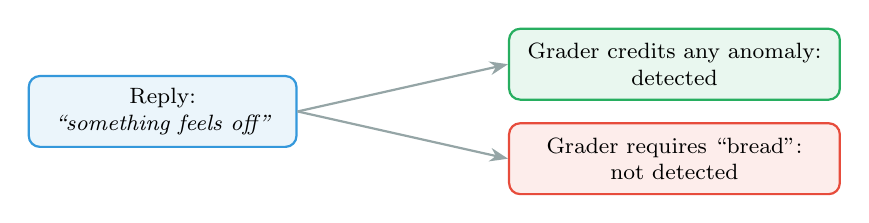
\begin{tikzpicture}
  \node[boxS=report,minimum width=3.4cm] (r) at (0,0) {Reply:\\{\footnotesize\itshape ``something feels off''}};
  \node[boxS=pass,minimum width=4.2cm] (g1) at (6.5,0.6) {Grader credits any anomaly:\\detected};
  \node[boxS=fail,minimum width=4.2cm] (g2) at (6.5,-0.6) {Grader requires ``bread'':\\not detected};
  \draw[-{Stealth},thick,neutral] (r.east) -- (g1.west);
  \draw[-{Stealth},thick,neutral] (r.east) -- (g2.west);
\end{tikzpicture}
\end{center}

{\footnotesize Michel calls the grader's choice the criterion content.}
\end{frame}

\begin{frame}[label=changmodel]{Fixed points and comparability in a model}
\begin{columns}[T]
\begin{column}{0.48\textwidth}
{\small\textbf{Fixed points}}\\[0.3em]
{\footnotesize A paper that uses injected vectors as its reference assumes the injected state is the same across layers, strengths and prompts. Chang's boiling point is the case in which an assumed fixed point turned out to depend on unspecified conditions.}
\end{column}
\begin{column}{0.48\textwidth}
{\small\textbf{Comparability as a minimal check}}\\[0.3em]
{\footnotesize Runs of one report procedure under different seeds, paraphrases or temperatures are thermometers of one type. The principle of single value requires that they agree about one state of one model.}
\end{column}
\end{columns}

\vspace{0.3em}
\begin{center}
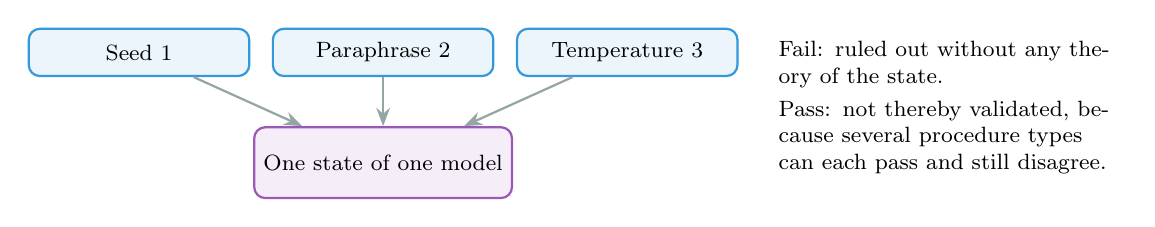
\begin{tikzpicture}
  \node[boxS=report,minimum height=0.6cm] (a) at (0,0) {Seed 1};
  \node[boxS=report,minimum height=0.6cm] (b) at (3.1,0) {Paraphrase 2};
  \node[boxS=report,minimum height=0.6cm] (c) at (6.2,0) {Temperature 3};
  \node[boxS=state] (s) at (3.1,-1.4) {One state of one model};
  \draw[-{Stealth},thick,neutral] (a) -- (s);
  \draw[-{Stealth},thick,neutral] (b) -- (s);
  \draw[-{Stealth},thick,neutral] (c) -- (s);
  \node[font=\footnotesize,align=left,text width=4.3cm,anchor=west] at (8.0,-0.7) {Fail: ruled out without any theory of the state.\\[0.3em]Pass: not thereby validated, because several procedure types can each pass and still disagree.};
\end{tikzpicture}
\end{center}
\end{frame}

\begin{frame}[label=itermodel]{Iteration in a model}
Chang's method, applied to concept injection:

\vspace{0.4em}
\begin{center}
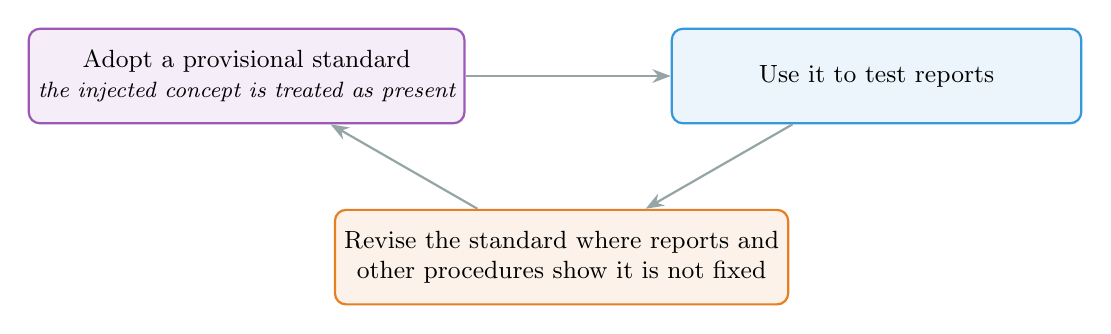
\begin{tikzpicture}
  \node[boxL=state] (a) at (0,0) {Adopt a provisional standard\\{\footnotesize\itshape the injected concept is treated as present}};
  \node[boxL=report] (b) at (8,0) {Use it to test reports};
  \node[boxL=bias] (c) at (4,-2.3) {Revise the standard where reports and\\other procedures show it is not fixed};
  \draw[-{Stealth},thick,neutral] (a) -- (b);
  \draw[-{Stealth},thick,neutral] (b) -- (c);
  \draw[-{Stealth},thick,neutral] (c) -- (a);
\end{tikzpicture}
\end{center}

\vspace{0.5em}
{\small This is the thermometer story again: the starting standard is accepted without proof, and what justifies it later is the record of corrections it made possible.}
\end{frame}

\begin{frame}[label=extmodel]{Extending ``introspection'' to models}
Carrying ``introspection'' from people to models is a metrological extension.

\vspace{0.5em}
\begin{center}
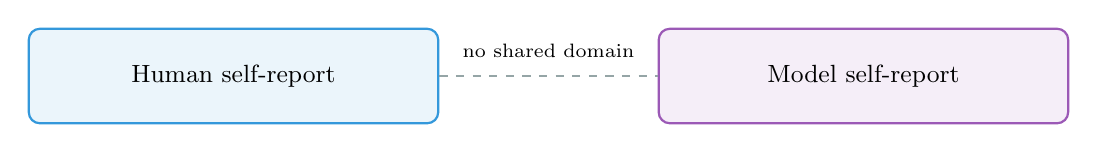
\begin{tikzpicture}
  \node[boxL=report] (h) at (0,0) {Human self-report};
  \node[boxL=state] (m) at (8,0) {Model self-report};
  \draw[dashed,thick,neutral] (h) -- node[above,yshift=3pt,font=\scriptsize,text=black]{no shared domain} (m);
\end{tikzpicture}
\end{center}

\vspace{0.5em}
\begin{itemize}\setlength\itemsep{5pt}
  \item {\small \textbf{Existence} (Michel): does the model have the state the report is about?}
  \item {\small \textbf{Overlap}: human and model self-report share no domain, so neither overlap condition can do any work.}
  \item {\small \textbf{Conformity} (Chang) carries the weight: the new standard should agree with whatever meaning ``introspection'' already has when applied to models.}
\end{itemize}
\end{frame}

\begin{frame}[label=limits]{Where the analogy stops}
\begin{itemize}\setlength\itemsep{1pt}
  \item {\small \textbf{No guaranteed convergence.} Chang's iterations ran for two centuries across many laboratories and converged on a quantity that thermodynamics later explained. Nothing guarantees that introspection measures converge on one quantity. Tal's individuation problem allows that they measure several quantities or none.}
  \item {\small \textbf{No trusted starting point.} Sensation of hot and cold had a range in which it was trusted. No such starting principle exists yet for model self-report.}
  \item {\small \textbf{No background theory.} Tal's cases, such as temperature and frequency, have theories that fix how they relate to other quantities. For internal states of a model there is none. Tal allows pre-theoretical assumptions in its place.}
  \item {\small \textbf{No independent standards.} Tal's standards are kept by institutions independent of the instruments they calibrate. Here the researchers construct the ground truth, and a judge model may score the replies.}
\end{itemize}
\end{frame}

\begin{frame}[label=summary]{Summary}
\begin{center}
{\footnotesize\renewcommand{\arraystretch}{1.05}\setlength{\tabcolsep}{4pt}
\begin{tabular}{>{\raggedright\arraybackslash}p{3.1cm}>{\raggedright\arraybackslash}p{7.4cm}>{\raggedright\arraybackslash}p{2.4cm}}
\toprule
\textbf{Idea} & \textbf{Question for an introspection experiment} & \textbf{Card stage} \\
\midrule
Indication, outcome & What is read off the reply, through which model? & Instrument \\
Fixed points & Does the injected state vary with layer or strength? & Calibration \\
Kinds of calibration & Is the report pathway modeled, or only reply rates? & Calibration \\
H1--H3 & Why do report and probe disagree? & Comparability \\
Comparability & Do runs of one procedure agree about one state? & Comparability \\
Robustness condition & Do diverse procedures agree within uncertainty? & Comparability \\
Metrological extension & Does the model have the state the report is about? & Validity conditions \\
\bottomrule
\end{tabular}
}
\end{center}
\end{frame}

\begin{frame}[label=reading]{Reading}
\small
\begin{itemize}\setlength\itemsep{0pt}
  \item \href{https://academic.oup.com/book/5530}{Chang, \emph{Inventing Temperature}} (2004): nomic measurement, comparability, single value, epistemic iteration, metrological extension.
  \item \href{https://plato.stanford.edu/entries/measurement-science/}{Tal, Measurement in Science} (SEP, 2020): the two-level account; coordination and nomic measurement named together.
  \item \href{https://philpapers.org/rec/TALCMT}{Tal, Calibration: Modelling the measurement process} (2017): three kinds of calibration; the generalized robustness condition.
  \item \href{https://philpapers.org/rec/TALIQ}{Tal, Individuating quantities} (2019): H1--H3; unity through idealization.
  \item \href{https://iopscience.iop.org/article/10.1088/1742-6596/772/1/012001}{Tal, How does measuring generate evidence?} (2016): outcomes as evidence through epistemic security.
  \item \href{https://philpapers.org/archive/MICCIC-2.pdf}{Michel, Calibration in Consciousness Science} (2021): calibration against an inaccurate procedure.
  \item \href{https://580d4178-4a2a-40ee-b753-91905f0859e6.filesusr.com/ugd/b898ea_5e898d22d16b4ba89c07c379485770ed.pdf}{Michel, Validity drifts in psychiatric research} (2024): existence condition; validity drift.
\end{itemize}
\end{frame}

\end{document}
